Die Framework Anwendung soll nur OCPP-Schnittstelle benutzen. 
Die HTTP- und Filesystem- Schnittstelle werden gar nicht gebraucht.
Die Datenbank-Schnittstelle soll simuliert werden, da es gewünscht wird, 
manche Informationen zu speichern um sie später verwenden bzw. auswerten zu können.

Die Anwendung lässt sich wie folgt darstellen 
(Die blaue Farbe stellt simulierte Komponenten dar, die schwarze Farbe stellt fehlende Komponente dar):

\import{./images/solutions}{Framework}

\newpage
Das Framework wird von Dritten benutzt. Aus diesem Grund benötigt es ein gutes Interface, 
das als Fassade (siehe Kapitel \ref{kap:gof:facade}) 
zu der komplexen Struktur in der Abbildung \ref{fig:solutionFramework} dient.
Die allgemeinen Regeln der Aufbau einer Framework-Anwendung sind im Kapitel \ref{kap:useFrameworkAndLibrary} beschrieben.

Die Struktur des Frameworks als Klassendiagramm sieht wie folgt aus:
\begin{figure}[H]
    \centering
    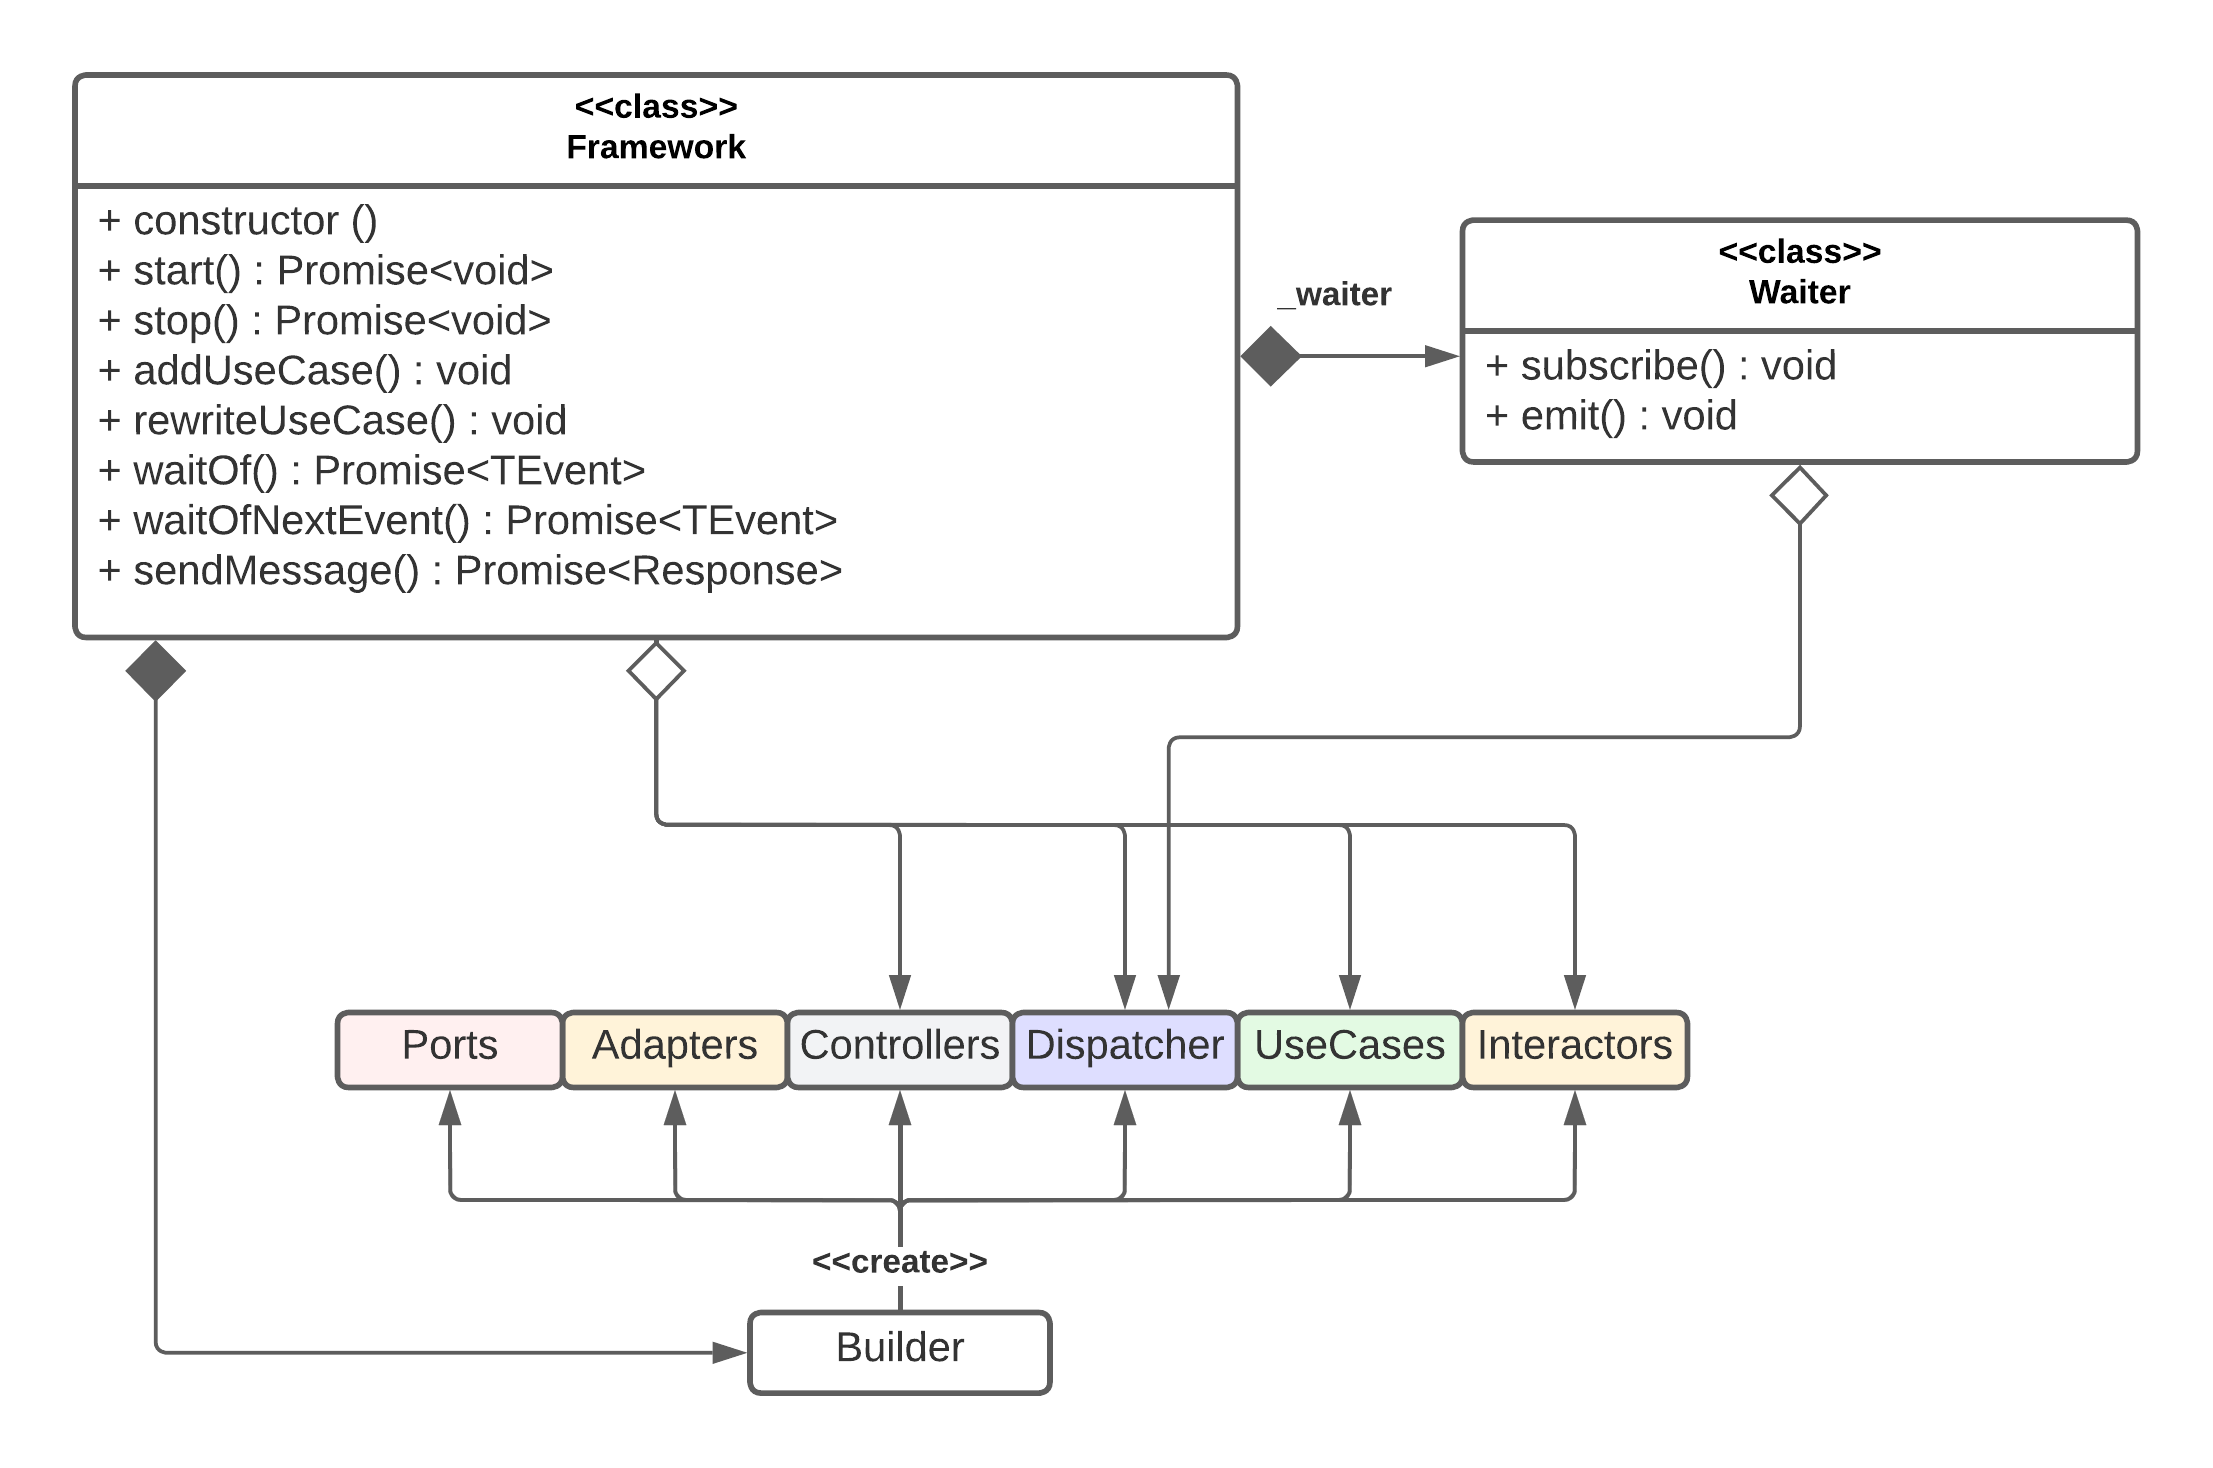
\includegraphics[width=1\textwidth]{./images/FrameworkKlassenDiagramm.png}
    \caption[Struktur des Frameworks]{Struktur des Frameworks}
    \label{fig:FrameworkStruktur}
\end{figure}

Das Interface des Frameworks besteht aus folgende Methoden:
\begin{itemize}
    \item start
    \item stop
    \item addUseCase
    \item rewriteUseCase
    \item waitOf
    \item waitOfNextEvent
    \item sendMessage
\end{itemize}

Jeder Test lässt sich in vier Phasen unterteilen, jede Methode bzw. 
Funktion des Frameworks soll einer dieser Phasen zugeordnet werden.
In der nachfolgenden Abbildung \ref{fig:TestFlow} 
ist eine Zuordnung der Methoden zu jeweiliger Phase in Form eines Ablaufdiagramms zu sehen:

\begin{figure}[H]
    \centering
    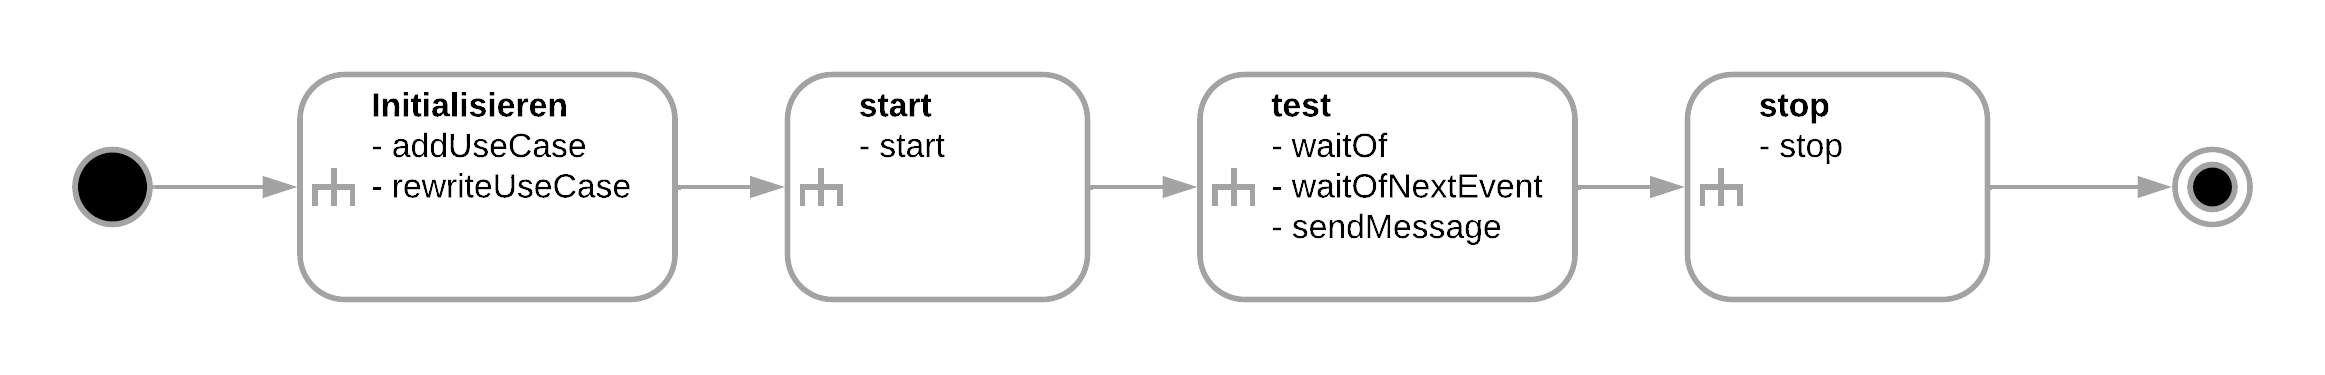
\includegraphics[width=1\textwidth]{./images/TestAblauf.png}
    \caption[Ablaufdiagramm eines Tests]{Ablaufdiagramm eines Tests}
    \label{fig:TestFlow}
\end{figure}